\chapter{Parallel Computing}
\label{ch:parallel_computing}
\dictum[Immanuel Kant]{%
	Sapere aude! Habe Mut, dich deines eigenen Verstandes zu bedienen! }%
\vskip 1em
%\section{Introduction}
\lettrine[lines=3,lhang=0.33,lraise=0,loversize=0.15]{T}{his} chapter briefly introduces  some of  the main concepts and technologies of parallel computing used thoughout this work.
It also contains a description of the Flynn's categorization of parallel architectures and a description of \textsc{OpenMP}, \textsc{OpenCL} together with examples of their usage and applications.

%manca MPI 

\section{Introduction and Motivations}
Traditionally performance improvements in computer architectures have come from cramming ever more functional units onto silicon, increasing clock speeds and transistors number.
Moore's law, shown in Figure \ref{fig:moore}, states that the number of transistors that can be placed inexpensively on an integrated circuit will double approximately every two years.
Coupled with increasing clock speeds, CPU performance has until recently scaled likewise.
But it is important to acknowledge that this trend cannot be sustained indefinitely or forever.
Increased clock speed and transistors number require more power and consequently, generate more heat.
Although the trend for transistor densities has continued to increase steadily, clock speeds began to slow circa 2003 at about $3$GHz.
If we apply Moore’s law type thinking to clock-speed performance, it should be able to buy at least $10$GHz CPUs. 
However, the fastest CPU available at the time of writing is $\approx 4.0 GHz$.
\begin{figure}[!htbp]
		\hspace*{-1.8cm}
\centering
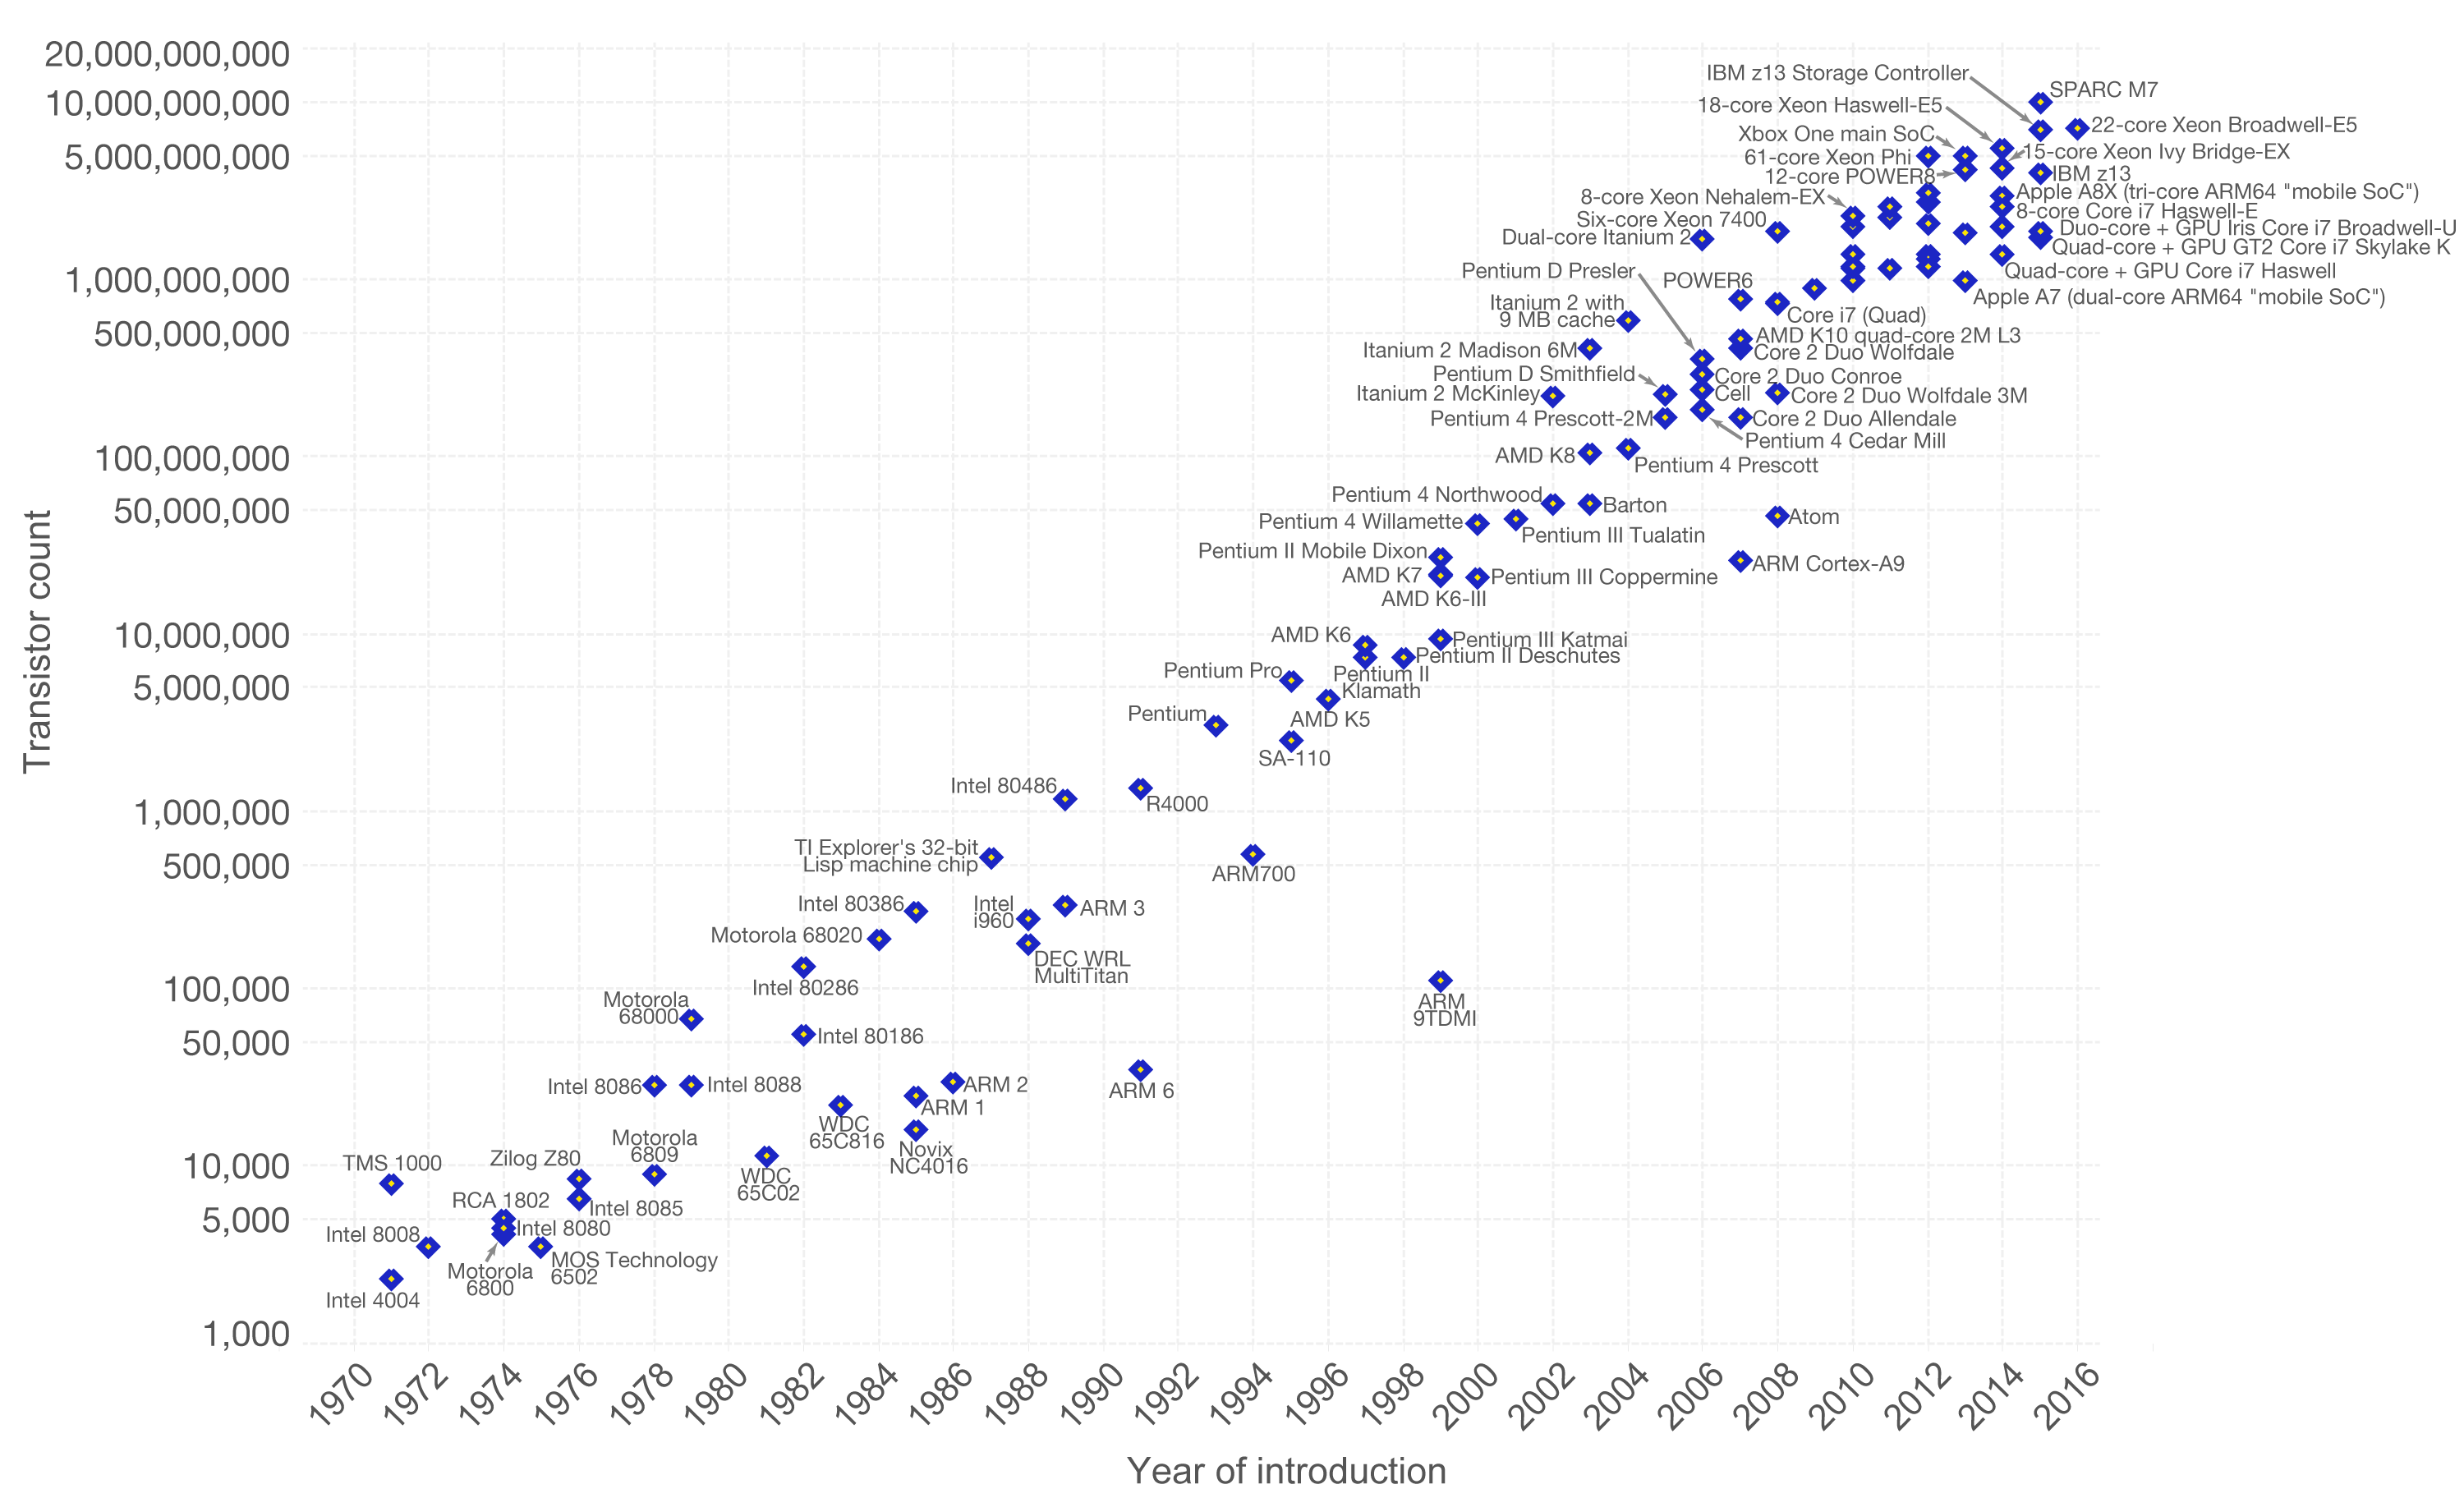
\includegraphics[width=1.2\textwidth]{./images/parallel_programming/moore_law2}
\caption[Moore's Law regarding CPUs transistors number.]{Moore's Law regarding CPU transistors number. \textsc{Intel} co-founder, Gordon Moore in 1695 observed that number of transistors in integrated circuits doubled each year. Although the pace has slowed in recent times, the number of transistors per square centimeter has since doubled approximately every 18 months. This is used as the current definition of the law. It is expected to hold true until 2020-2025. Note the logarithmic vertical scale. The almost linear trend correspond to an exponential growth.
}
\label{fig:moore}
\end{figure}
At same point the gain in performance in terms of clock speeds fails to increase proportionally with the additional efforts needed to overcome heat dissipation problems that in turn, become more and more important and challenging.
The heat emitted from the modern processor, measured in power density rivals the heat of a nuclear reactor core (see Figures \ref{fig:tempCPU} and \ref{fig:tempCPU_thermal})!
Additionally, the transistor resolution on the wafer is not far from from its physical limit (at the atomic scale), preventing further improvements.
But the power demand did not stop in these year, and is not going to stop in the near future, and from these reason comes the necessity of relying heavily on parallel architectures.
Today, the dominating trend in commodity CPU architectures is multiple processing cores mounted on a single die operating at "reduced" clock speeds  sharing resources and memory with each other.
Multi-core (2,4,8,12, up to 40) CPUs on a desktop PC at home or at the office are ubiquitous at the point that is even hard to be able to buy a single core device.
Even smart-phones are proper multi-core machines; for instance, the popular mobile CPU, the \textit{Snapdragon 835}, manufactured by \textit{Qualcomm} is a $8 \times$ cores, each of them with a clock speed up to $2.45$ \si{GHz}.
\begin{figure}[!htbp]
\centering
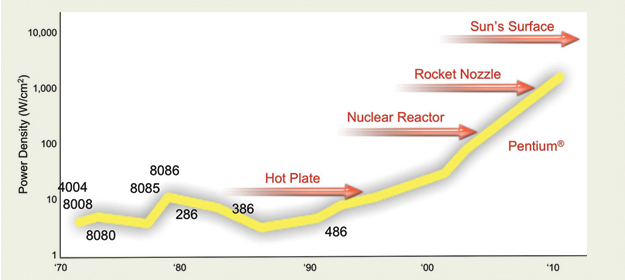
\includegraphics[width=1.0\textwidth]{./images/parallel_programming/temperatureCPU}
\caption[Temperature density of CPUs over the years.]{Integraed Circuits power density over the years. Note  that since 2000s power density is higher in CPUs than in nuclear reactors. This clearly shows that this trend is not sustainable.}
\label{fig:tempCPU}
\end{figure}
Lot of efforts have been put during these years in order to mitigate and overcome the limits that the sequential computer architecture has which its three main components impose:
\begin{enumerate}
\item Processor (Cores, branch prediction etc.)
\item Memory (Ram, Caches, Registers etc.)
\item Communication system i.e. datapaths,usually buses (PCI or SCSI)
\end{enumerate}
All three components present bottlenecks that limit the overall computing performance capability of a system.
Caches, low-latency high bandwidth and small capacity high speed memories, for example can hide latency of DRAM storing the fetched data and serving subsequent requests of the same memory (or neighboring) locations\footnote{The fraction of the data served by the various caches is commonly refeered to as \textit{\textbf{hit rate}}.}.
But one of the most important innovation that addresses these bottlenecks is \textbf{multiplicity} (in processors, memories and datapaths) that allows to improve the overall performance of a system and thus extending the size of the problems that a computer can solve.
Hardware multiplicity has been organized in several manners during the years, giving birth to a variety of parallel computer architectures.
\begin{figure}[!htbp]
	\centering
	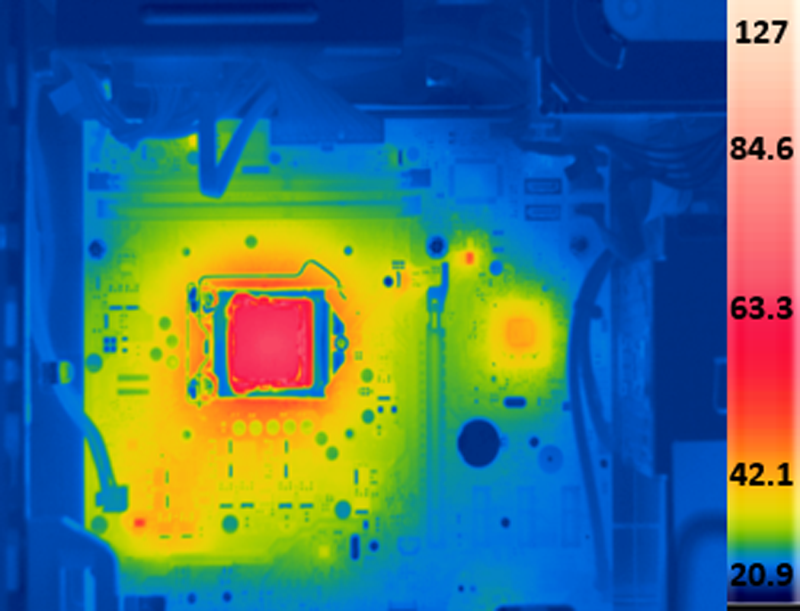
\includegraphics[width=0.5\textwidth]{./images/parallel_programming/heat_cpu}
	\caption[CPU and Motherboard Temperature.]{Thermal camera image of a modern CPU showing that the whole CPU heat is concentrated in a small part of the wafer i.e. power density is. is very high in some areas.}\label{fig:tempCPU_thermal}
\end{figure}

\section{Parallel Architectures - Flynn's taxonomy}
\label{sec:flynn_tax}
A number of definitions and classifications have been proposed  over the years in order to categorize parallel systems, the majority of them are mostly based on the adopted hardware configuration or on the logical approach in handling and implementing the parallelism.
Among all, \textit{Flynn}'s  taxonomy \cite{flynn:1972,duncan:1990} is probably the most famous and it is also well accepted by the scientific community, therefore introduced briefly in this section.

Flynn's classification is based on the notion of  \textit{stream of information}.
Two types of information flow into the processor: \textbf{instructions} and \textbf{data}.
Conceptually they can be separated into two independent streams.
A coarse classification can be made taking in account only the number of streams of both instructions and
data that an architecture can manage concurrently (see figure \ref{fig:parallelClassification1}).
Flynn's taxonomy classifies machines according to whether they have one or more streams of each type.
\begin{table}
		\caption[Flynn's Parallel architecture taxonomy]{Flynn's Parallel architecture taxonomy.}
	\label{fig:parallelClassification1}
	\begin{tabular}{lcccc}\toprule
		&\multicolumn{2}{c}{\textbf{\textsf{Single Instruction}}}&\multicolumn{2}{c}{\textbf{\textsf{Multiple Instructions}}}
		\\\cmidrule(r){2-3}\cmidrule(r){4-5}   
		&\textbf{\textsf{Single Data}}&\textbf{\textsf{Multiple Data}}&\textbf{\textsf{Single Data}}&\textbf{\textsf{Multiple Data}}\\\midrule
		& \textsc{sisd} & \textsc{misd}
		& \textsc{misd} & \textsc{mimd}
		\\\bottomrule
	\end{tabular}

\end{table}
Flynn's classifies architectures into four main categories:
\begin{description}
\item[SISD:] \textit{\textbf{Single}} instruction \textit{\textbf{Single}}
data.\hfill\\
No parallelism in either instruction or data streams.
Each arithmetic instruction initiates an operation on a data item taken from a single stream of data elements.
A single control unit fetches a single instruction from the memory.
Mainframes belong to this category.
\item[SIMD:] \textit{\textbf{Single}} instruction \textit{\textbf{Multiple}} data. \hfill \\ 
Data parallelism. The same instruction is executed on a batch of different data.
The control unit is responsible for fetching and interpreting one instruction at a time.
When it encounters an arithmetic or an other data ALU instruction, it broadcasts the instruction
to all processing elements (PE), which then all perform the same operation in unison.
For example, the instruction might be \texttt{add R3,R0.}.
Each PE would add the contents of its own internal register R3 to its own R0.
This is how stream processors work, for example, data elements are distributed across all available data memories. and the same instruction executed on each PE.
\texttt{SSE} and \texttt{AVX} extensions to the $x86$ processors family is an example of such parallelism.
One single instruction can operate on up to $512$ byte of data (see Figure \ref{fig:SSEvectorization} and Listing \ref{code:avxvectorization}).
SIMD exploits \textbf{data and spatial parallelism} in a synchronous manner.
\lstset{language=[OpenCL]C,frame=tb,
	caption=[Multiplying eight floats using Intel AVX vectorization.]{Multiplying eight floats of one array by eight floats of a second array and add the result to a third array. Serial and SIMD (AVX2) code examples. Note that the AVX2 intrinsic function \texttt{\_\_mm256\_fmadd\_ps} processes twentyfour floats, but it does not map to a single instruction (see Figure \ref{fig:SSEvectorization}). Instead, it executes three instructions: \texttt{vfmadd132ps}, \texttt{vfmadd213ps}, and \texttt{vfmadd231ps}. Despite this, it executes quickly and it is much faster than looping through the individual elements.}, 
	label=code:avxvectorization, 
	basicstyle=\footnotesize\ttfamily,
	keywordstyle=\color{ultramarine}\ttfamily,
	stringstyle=\color{rosemadder}\ttfamily,
	commentstyle=\color{gray}\ttfamily,
	backgroundcolor=\color{gray!5}, 
	numbers=left,numbersep=3pt,, 
	numberstyle=\tiny\ttfamily\color{gray},
	morekeywords=[2]{__m256,_mm256_fmadd_ps},
	%keywordstyle=[2]\color{violet},
}
\begin{lstlisting}
//adds 8 floats in a serial fashion. One at the time in 8 different steps
void multiply_and_add(const float* a, const float* b, const float* c, float* d) {  
	for(int i=0; i<8; i++) {
		d[i] = a[i] * b[i];
		d[i] = d[i] + c[i];
	}
}
//A single instruction adds 8 floats in a SIMD fashion
__m256 multiply_and_add(__m256 a, __m256 b, __m256 c) {
	return _mm256_fmadd_ps(a, b, c);
}
\end{lstlisting}
\begin{figure}[!htbp]
	\centering
	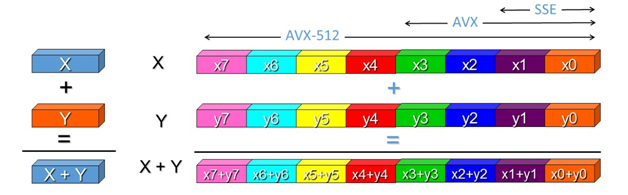
\includegraphics[width=1.0\textwidth]{./images/parallel_programming/vectorization_example}
	\caption{Example of vectorization with Intel SSE and extension.}
	\label{fig:SSEvectorization}
\end{figure}

\item[MISD:] \textit{\textbf{Multiple}} instruction \textit{\textbf{Single}} data. \hfill \\ 
Multiple instruction operating on the same single data stream  (ee Figure \ref{fig:MISD}). It is a class of system very unusual. No machines in this category have been commercially successful or had any impact on computational science. 
A type of computer  that fits the MISD description is the so called \textit{systolic array} \cite{fortes:1987,kung:1984} which consists of a network of pipelined primitive computing nodes or processors. 
\begin{figure}[!htbp]
	\centering
	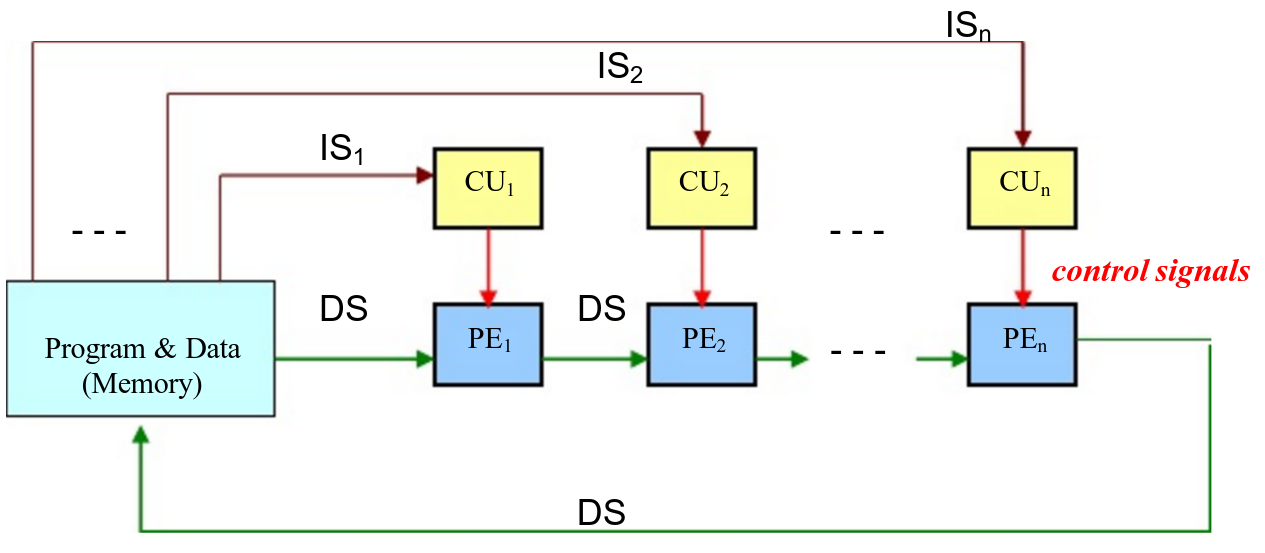
\includegraphics[width=1.0\textwidth]{./images/parallel_programming/MISD}
	\caption{MISD machine schematization. Each processor $CU_i$ has its own instruction flow and all operates on the same data.}
	\label{fig:MISD}
\end{figure}
 
\item[MIMD:] \textit{\textbf{Multiple}} instruction \textit{\textbf{Multiple}} data. \hfill \\
Multiple instructions operating independently on multiple data streams.
Most modern computers belogn to this family. A MIMD machine is an example of a true multiprocessor and are often employed to perform the so called \textit{Single Program Multiple Data} computation where each independent processor executes the same program.
Note that modern machine also exposes SIMD capability within each instruction stream.
MIMD architecture can be further divided by considering the  layout organization of memories:
\begin{description}
	\item [Shared Memory (modern CPUs)] where each processors shares the same memory address space and are interconnected by shared buses. 
	Shared memory architecture are usually shipped as \textit{Symmetric Multi Processors} (SMP) since each of them is usually identical in computational and access to resources capabilities, and the OS kernel can run on any of them in contrast to \textit{Asymmetric Multiprocessor}s where there is a master-slave relationship  among the group of processors.
	According to whether subsets of processors have a dedicated/private memory module we can categorize SM architectures in:	
	\begin{itemize}
		\item UMA (Uniform Memory Access) : Identical processors with equal
		access time to memory (see figure \ref{fig:UMA_NUMA}).
		Also known as \textit{Cache Coherent UMA} (CC-UMA), because the
		hardware ensures that all the processor can see a modification in memory performed by one of them.
		\item NUMA (Non Uniform Memory Access): Usually different groups
		 Symmetric multiprocessors (SMP), group of usually not more than 32 processors communicating via buses, are inter-connected, and processors belonging to different SMP can access the memory spaces of each others. Time for memory access is not uniform because the cost for a communication among SMP is higher than a intra-SMP one.
		 As for UMA, if a cache coherence mechanism  is present, then this architecture is called \textit{CC-NUMA}.
		 \begin{figure}[b]
			\caption[Shared memory architectures.]{UMA and NUMA shared memory architecture.}
			\label{fig:UMA_NUMA}
			\centering
			\begin{subfigure}[b]{0.5\textwidth}
				\centering
				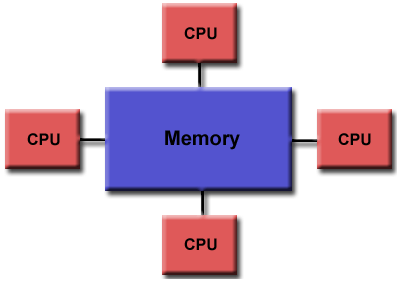
\includegraphics[width=0.92\textwidth]{./images/parallel_programming/shared_mem}
				\caption[]{}%
			\end{subfigure}%
			\begin{subfigure}[b]{0.5\textwidth}
				\centering
				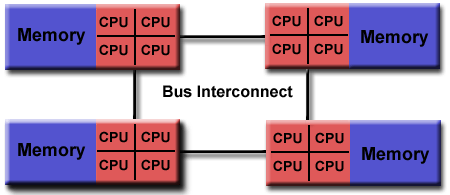
\includegraphics[width=0.92\textwidth]{./images/parallel_programming/numa}
				\caption[]{}%
			\end{subfigure}%

		\end{figure}
	\end{itemize}
	SM architecture provides an easy perspective to memory,	data sharing across processors and parallelism since no explicit communication is involved. Memory accesses and communications are fast due to the proximity of memory to CPUs, but it is not scalable because adding more CPUs to the pool can geometrically increases the traffic on the bus and makes cache management harder. Additionally, ensuring the correctness of accesses to global memory, in order to avoid race-conditions, is up to the programmer.
	As an example of real world SM modern processor, Figure \ref{fig:intelPhi} shows the Intel \textit{Knights Landing} architecture for the Intel Phi processor family which is armed with 72 cores, $8$ billions transistors at \SI{14}{\nano\metre}, AVX-512 and is able to executes 240 threads simultaneously.
	Coupled with this architecture many software model can be used to program
	SM machines. Among all, the most used are:
	\begin{itemize}
		\item Threads; Lightweight processes but with same PID (e.g. pthreads)
		\item Compiler preprocessor directives; A standard language with preprocessor directives to the compiler that is capable of converting the serial program in a parallel one without any (or very few) interventions or hints by the programmer (e.g. \texttt{OpenMP}, introduced in Section \ref{sec:openmp}).		
	\end{itemize}	
	\item [Distributed Memory] 	Different systems, and hence, different multiprocessors connected via some kind of network (see Figure \ref{fig:distribuiteMemory}), usually high speed networks such as gigabit \textsc{Ethernet} \cite{Spurgeon:2000:EDG:336070}, \textsc{InfiniBand} \cite{Shanley:2002:INF:579371} and \textsc{Myrinet} \cite{Boden:1995:MGL:623261.623898}, where the memory space in one processor does not map to another's one.
	Each of them operate independently on its memory address, so changes are not reflected on memory spaces of the others. Explicit communication is required between processors with synchronization under the programmer responsibility.
	This architecture  is very scalable and there is not  overhead in maintaining	cache coherency. 	
	The most used paradigm for programming distributed memory machines is the
	message passing for which the \textit{Message Passing Interface} (\texttt{MPI}\footnote{\url{http://www.mpi-forum.org/}}) \cite{Forum:1994:MMI:898758,Gropp:1999:UMA:555151} is the \textit{de facto} industrial and academic standard.
	
	\item[Hybrid Systems] As the name suggest a system belonging to this category, is a mix of architectures. Only a limited number of  processors, say $N$, have access to a common amount of shared memory. They are  inter-connected to the others groups via network. Each group  usually is an agglomerate of many computing cores (SMP).
		Hybrid systems of the kind described in this section are usually programmed using a combination of the message passing model (\texttt{MPI}) with the threads model (\texttt{OpenMP}) in which:
		\begin{itemize}
			\item threads perform computationally intensive task, using local
			\textbf{on-node} memory space, taking advantage of spatial locality of data (via vectorization/AVX for instance) and 
			\item communications between processes on different nodes occurs over network using \texttt{MPI} (see figure \ref{fig:hybridMemory}).
	\end{itemize} 
\end{description}
 
 \begin{figure}
 	\centering
 	\begin{subfigure}{0.55\textwidth}
 		\centering
 			\caption{Hybrid memory architecture (each processor is milti-core)}
 		\label{fig:hybridMemory}
 		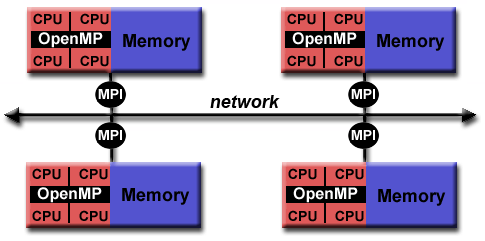
\includegraphics[width=0.95\textwidth]{./images/parallel_programming/hybrid_model}
 	
 	\end{subfigure}%
 	\begin{subfigure}{0.45\textwidth}
 		\centering
 		\caption{Distributed memory architecture.}
 		\label{fig:distribuiteMemory}
 		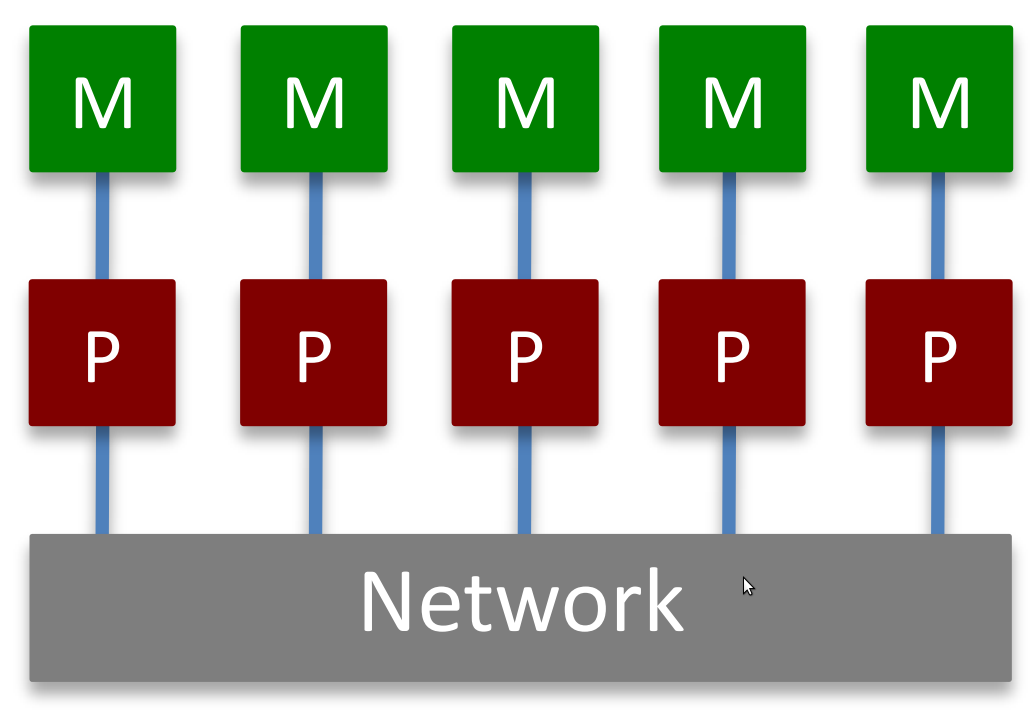
\includegraphics[width=0.92\textwidth]{./images/parallel_programming/distribuitedMemory}
 	\end{subfigure}%
 \end{figure}

\begin{figure}
	\centering
	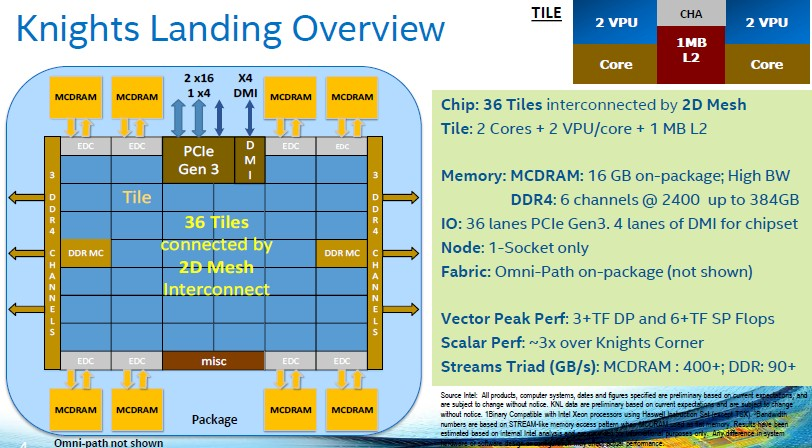
\includegraphics[width=1.0\textwidth]{./images/parallel_programming/xeonphi}
	\caption{Xeon Phi, Intel Knight Landing architecture and technical specifications.}
	\label{fig:intelPhi}
\end{figure}



\section{The \texttt{OpenMP} Parallel Computing Paradigm for Shared Memory Computers}
\label{sec:openmp}
    \texttt{OpenMP} is a portable API providing compiler directives and library
    functions for shared memory parallel programming in \texttt{C/C++} and
    Fortran \cite{Chapman:2007:UOP:1370966} designed on top of \texttt{pthread} \cite{Nichols:1996:PP:237813}. It implements the
    multi-threaded \emph{fork-join}  programming model (see Figure \ref{fig:omp_fork-join}), where an initial (or master) thread forks a given number of new threads (team of threads), which share the resources of the parent process and run concurrently on the available processing cores.
    Threads created during the \textit{fork} phase can therefore
    rejoin to the master thread (join phase), and more \textit{fork-join}
    stages can occur in a typical execution of an \texttt{OpenMP} executable.
    The size of the teams can be controlled by an environment variable \texttt{OMP\_NUM\_THREADS}, set at runtime by using the \texttt{omp\_set\_num\_threads(n)} function or specified for each parallel region using \texttt{num\_thread(n)} in the \texttt{\#pragma omp parallel} directive (see Listing \ref{code:openmp_lock}).
\begin{figure}[H]
	\centering
	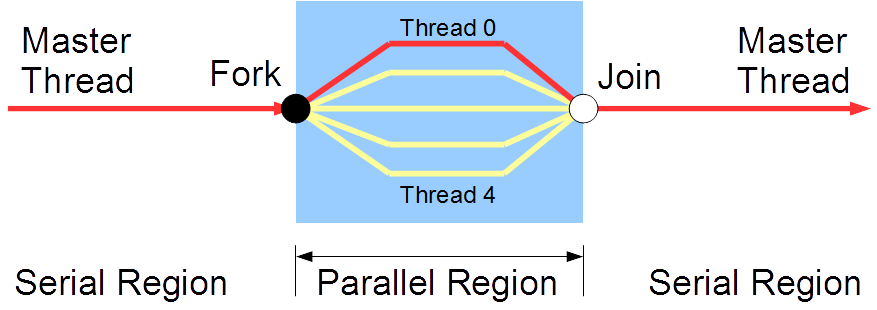
\includegraphics[scale=0.8]{./images/parallel_programming/omp_fork-join}
	\caption[\texttt{OpenMP} fork-join execution model.]
	{\texttt{OpenMP} fork-join execution model.
		\begin{inparaenum}
			\item OpenMP programs start with a single thread; the \textit{master thread} (\textit{Thread \#}$0$).
			\item At the starting point of a parallel region, \textit{master} creates team of parallel worker threads (\textbf{FORK}).
			\item Statements in the parallel block are executed in concurrently by every thread (master as well). 
			\item At end of parallel region, all threads \textbf{synchronize}, and join \textit{master} thread (\textbf{JOIN}).
		\end{inparaenum} Note that parallel regions can be nested.}
	\label{fig:omp_fork-join}
\end{figure}
    The \textit{fork-join} model allows for the selective parallelization of
    the original source code (e.g. loops), by leaving portions that
    are difficult to be parallelized or that would lead to negligible
    (or even worsening) improvements, unchanged with respect to the
    serial implementation.
    Numerical applications usually accomplish most of their work in a relatively small portion of their codebase, known as \textit{hotspots}. Those are the solely parts of an application that are worth parallelizing. Profilers and performance analysis tools are funamental and employed extensively during in order to identify such hotspots.   
    OpenMP can therefore effectively utilized to share the iterations of a loop within a pool of threads.
    
    By default, static scheduling is adopted where iterations are equally
    subdivided in chunks and statically allotted to threads in a
    round-robin policy. However, iterations can also be assigned to
    threads on demand, by using the \textit{dynamic} scheduling clause. In this
    manner, when a thread terminates processing its current chunk, it requests for a new one, usually resulting in better performance in the case where load is not well balanced across chunks.
    Scheduling can be specified using the \texttt{schedule} keyword in the \texttt{\#pragma omp for} directive.
    Static scheduling can be non-optimal in the case when different iteration take different amount of time to be executed. As an example consider the program in Listing \ref{code:scheduling_omp} in which each loop iteration causes the executing thread to sleep for a number of seconds equals to the number of the iteration. 
    \lstset{language=[OpenCL]C,
    	caption={Scheduling in OpenMP example. Note that specifying \textbf{static scheduling } is not needed since it is the default setting.}, 
    	label={code:scheduling_omp}, 
    	basicstyle=\ttfamily,
    	keywordstyle=\color{ultramarine}\ttfamily,
    	stringstyle=\color{rosemadder}\ttfamily,
    	commentstyle=\color{outerspace}\ttfamily,
    	backgroundcolor=\color{gray!5}, 
    	numbers=left, 
    	numberstyle=\tiny,
    	morekeywords=[2]{schedule,parallel,omp,pragma,num_threads,omp_get_thread_num,omp_destroy_lock,omp_unset_lock,omp_set_lock,omp_lock_t,omp_init_lock},
    	%keywordstyle=[2]\color{ultramarineblue}\ttfamily   	
    }
    \begin{lstlisting}
    #define CHUNK_SIZE (1)
    int main ( ) {
    	#pragma omp parallel for schedule(static,CHUNK_SIZE) num_threads(4)
    	for (int i = 0; i < N; i++) {
    		/* wait for i seconds */
    		sleep(i);    		
    		printf("Thread %d has completed iteration %d.\n", 
    				omp_get_thread_num( ), i);
    	}
    	/* all threads done */
    	printf("All done!\n");
    	return 0;
    }
\end{lstlisting}
Among the threads spawned by code in Listing \ref{code:scheduling_omp}, there is a great imbalance  in the number of seconds they will wait,  because the last thread executes the last chunk of iterations (which translates to longer sleep time).
\textit{Dynamic} scheduling can be applied in a case like this to improve the overall execution time. \texttt{OpenMP} assigns one iteration to each thread and when a thread completes its work, it is assigned the next iteration that has not been executed yet reducing execution time effectively. See table \ref{tab:scheduling_policies} for a complete list description of all kind of scheduling in OpenMP.

Moreover, \texttt{OpenMP} provides locking mechanism to serialize the access to shared variables by defining critical sections.
A lock must be firstly  initialized and then can be acquired or released.
When a thread  attempts to acquire a lock that is already be set by another
thread, its execution is suspended until the lock is released,
giving rise to performance degradation (or even to possible deadlock situations). 
However, a lock can also be queried in order to evaluate its state, without blocking the thread execution.
In thisway, if the lock is already set, the querying thread can do
perform other trasks, thus minimizing idle time.
See Listing \ref{code:openmp_lock} for an example of lock usage in OpenMP.
\begin{minipage}{1.0\textwidth}
\lstset{language=[OpenCL]C,
	caption={\texttt{OpenMP} lock acquisition, usage and destruction example. Note that the region of code between lines 6 and 8 is serialized.}, 
	label={code:openmp_lock}, 
	basicstyle=\ttfamily,
	keywordstyle=\color{ultramarine}\ttfamily,
	stringstyle=\color{rosemadder}\ttfamily,
	commentstyle=\color{outerspace}\ttfamily,
	backgroundcolor=\color{gray!5}, 
	numbers=left, 
	numberstyle=\tiny,
	morekeywords={#pragma,omp_destroy_lock,omp_unset_lock,omp_set_lock,omp_lock_t,omp_init_lock}
}
\begin{lstlisting}
omp_lock_t writelock;
omp_init_lock(&writelock);
#pragma omp parallel for num_threads(5)
for ( i = 0; i < x; i++ ){
// some stuff in a concurrent fashion
omp_set_lock(&writelock);
// one thread at a time stuff
omp_unset_lock(&writelock);
// some more  stuff in a concurrent fashion
}    
omp_destroy_lock(&writelock);
\end{lstlisting}
\end{minipage}   

    In addition to the data-type parallelization provided by the
    fork-join model, \texttt{OpenMP} aslo supports the functional-type
    parallelization, where different portions (called \textit{regions}) of code to be
    processed are assigned to different threads. In both cases, \texttt{OpenMP}
    parallelization of a code is straightforward, by hiding most
    low-level implementation details.
    Moreover, by using \texttt{OpenMP} it is
    possible to build the same source code to produce both parallel or
    sequential executable. In the latter case, the compiler simply
    ignores the \texttt{\#pragma omp} directives.
    \begin{table}
    	   	\begin{tabularx}{1.0\textwidth}{cX}
    		\rowcolor{gray!35}	
    		\heading{\textbf{Scheduling Kind}} &  \heading{\textbf{Description}} \\ \hline
    		\rowcolor{gray!15}
    		\texttt{\textbf{static}} & The loop is divided into equal-sized chunks of iterations. By default, chunk size is $\frac{iterations}{number\_of\_threads}$. If the chunk size is set to $1$, iteration are executed by the threads in a interleaved fashion.\\ \hline
    		\rowcolor{gray!5}
    		\texttt{\textbf{dynamic}} & chunk-sized block of iterations are internally queued. When a thread is ready to execute some work, it retrieves the next block  from the top of the queue. Note that by default chunk size is $1$. Managing the queue and assigning work to  to threads comes with an arrached overhead.\\ \hline
    		
    		\rowcolor{gray!15}
    		\texttt{\textbf{guided}} & similar execution policy  to \texttt{dynamic} but che chunk size decreases over time to better handle load imbalance between iterations. In this cake the optional parameter of the schedule construct specifies the minimum chunk size. By default it is equal to $\frac{iterations}{number\_of\_threads}$\\ \hline
    		
    		\rowcolor{gray!5}
    		\texttt{\textbf{auto}} & The compiler is free to decide any possible mapping of iteration to threads.\\ \hline
    		
    		\rowcolor{gray!15}
    		\texttt{\textbf{runtime}} & the scheduling policy is choosen at runtime and changes according to the environment variable \verb|OMP_schedule| \\ \hline
    	\end{tabularx}
    
    	\caption[OpenMP scheduling policies]{\texttt{\#pragma omp parallel for schedule(kind [,chunk size])} OpenMP scheduling kinds. The optional parameter (chunk size), when specified, must be a positive integer. }
    	\label{tab:scheduling_policies}
    \end{table}
    
    \subsection{General Purpouse GPU Computing - GPGPU}
    The concept of many processors working together in concert is not new in computer graphics. Since the demand generated by entertainment started to grow, multi-core hardware emerged in order to take advantage of the high amount of parallel work available in the process of generating and rendering and manipulation of $3D$ images.
    The main goal of the computer graphics is to render and then display $3D$ images onto the screen, which translates to refreshing pixels at rate of sixty or more $\si{Hz}$ \cite{Akenine-Moller:2002:RR:553838}.
    Each pixel has to be processed goes through a number of stages, and this process is commonly referred as to the \emph{graphic processing pipeline}.
    The peculiarity of this task is that the computation of each pixel is independent of the other's.
    This specific task is thus suitable for distribution over parallel processing elements as it can be categorized as  a \textbf{embarassingly, perfect} or \textbf{pleasingly} \textit{parallel} problem\cite{Foster:1995:DBP:527029} (see Section \ref{sec:opencal_julia} and Listing \ref{code:julia_set} at pages \pageref{sec:opencal_julia} and \pageref{code:julia_set} respectively, for an example of a perfectly parallel problem).
    To support extremely fast processing of large graphics data sets (which mainly consists of vertices and fragments), modern GPUs employ a stream processing model with parallelism.
    The game industry boosted the development of  GPUs, that offer today greater performance than CPUs and are improving faster too as shown in Figures  \ref{CPU-VS-GPU_GFLOP} and \ref{CPU-VS-GPU_MEMORY}.
    The reason behind the discrepancy in floating-point capabilities between CPU and  GPU is that GPUs are designed such that more transistors are devoted to data crunching and processing rather than caching, flow control, branch prediction, etc..
    Also note that memory bandwith is still one of the main advantages of GPU and Xeon Phi over CPUs architectures. The gap is getting wider thanks also to the introduction of High Bandwidth Memories (HBM), stacked memory by NVIDIA and MCDRAM for Xeon Phi \cite{Sodani:7477467,Jun:7939084}. 
    \begin{figure}[!htbp]
    	\centering
    	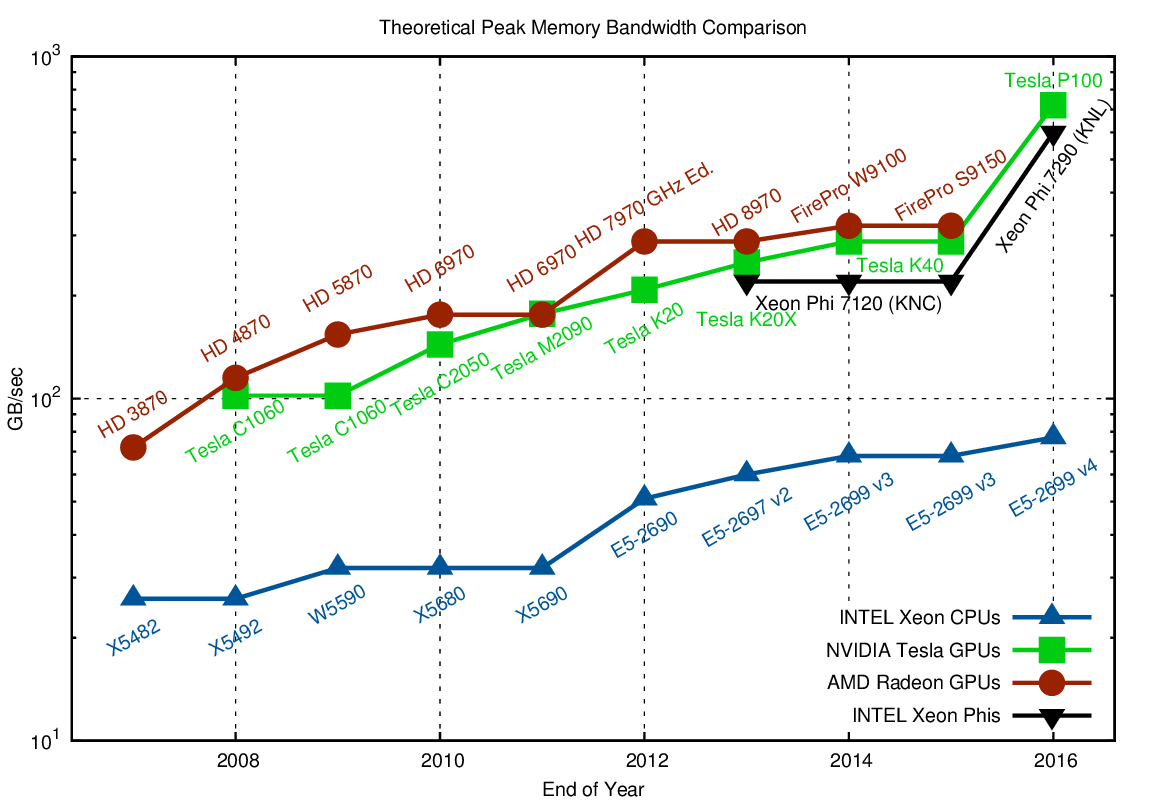
\includegraphics[width=1.0\textwidth]{./images/parallel_programming/memory-bandwidth}
    	\caption[\textsc{Intel} CPUs and \textsc{NVIDIA} GPUs memory bandwidth
    		chart]{Memory Bandwidth comparisong between \textsc{Intel} CPUs and \textsc{NVIDIA} chips over time. Higher is better.}
    		\label{CPU-VS-GPU_MEMORY}
    \end{figure}
    \begin{figure}[!htbp]
    	\centering
    	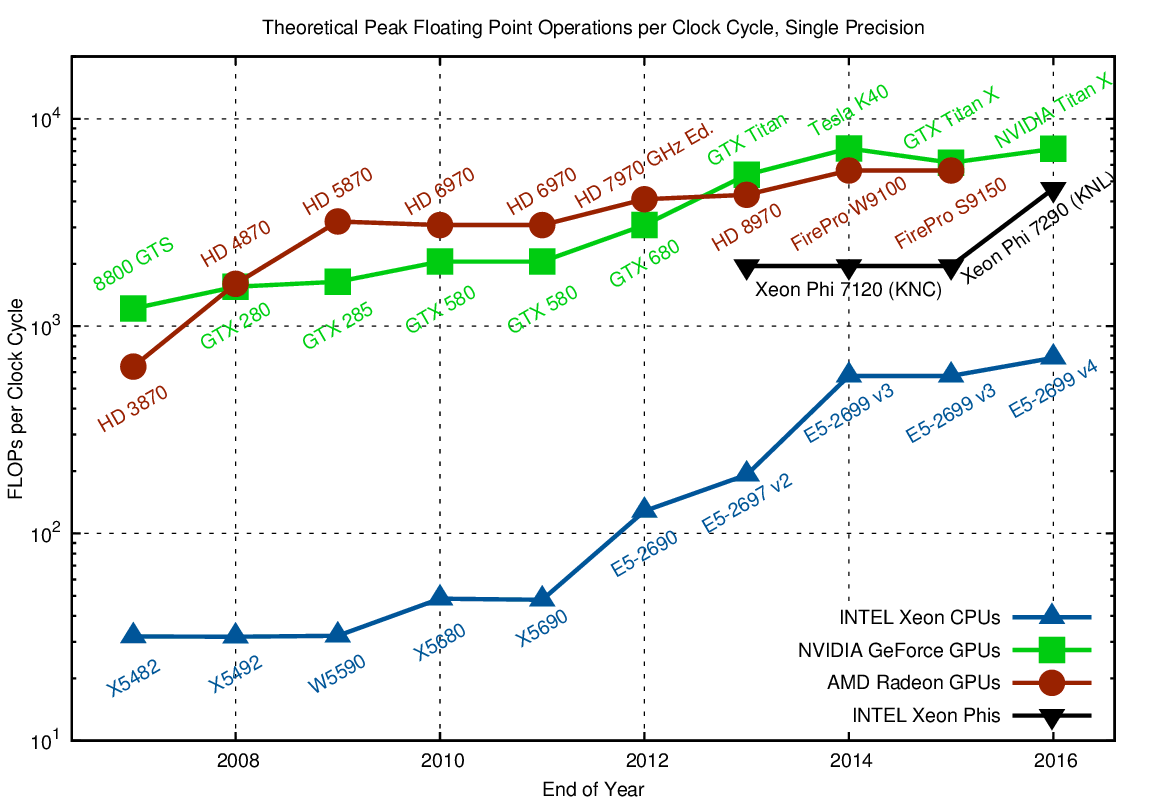
\includegraphics[width=1.0\textwidth]{./images/parallel_programming/cpu-vs-gpu}
    	\caption[Performance comparison (FLOPs) between CPU and modern accelerators (\textsc{NVIDIA}, \textsc{Intel} and \textsc{AMD})]{Performance comparison (FLOPs) between CPU and modern accelerators (\textsc{NVIDIA}, \textsc{Intel} and \textsc{AMD}) over time. When Double precision is considered, relative performance between the considered hardware does not change. Higher is better.}\label{CPU-VS-GPU_GFLOP}
    \end{figure}
    Nowadays, GPU are widely used for general purpouse computing. The Top $500$ supercomputers  ranking \footnote{\url{http://www.top500.org/statistics/list/}}  \cite{Strohmaier:2006:TS:1188455.1188474} is dominated by massively parallel computer, built on top of superfast networks and millions of sequential CPUs working in concert.
    But as the industry is developing even more powerful, programmable and capable GPUs in term of \si{\giga FLOPS},  we see that they begin to offer advantages over traditional cluster of computers in terms of economicity and scalability as depicted in Figure \ref{gflops-per-watt-sp}.
        \begin{figure}[!htbp]
    	\centering
    	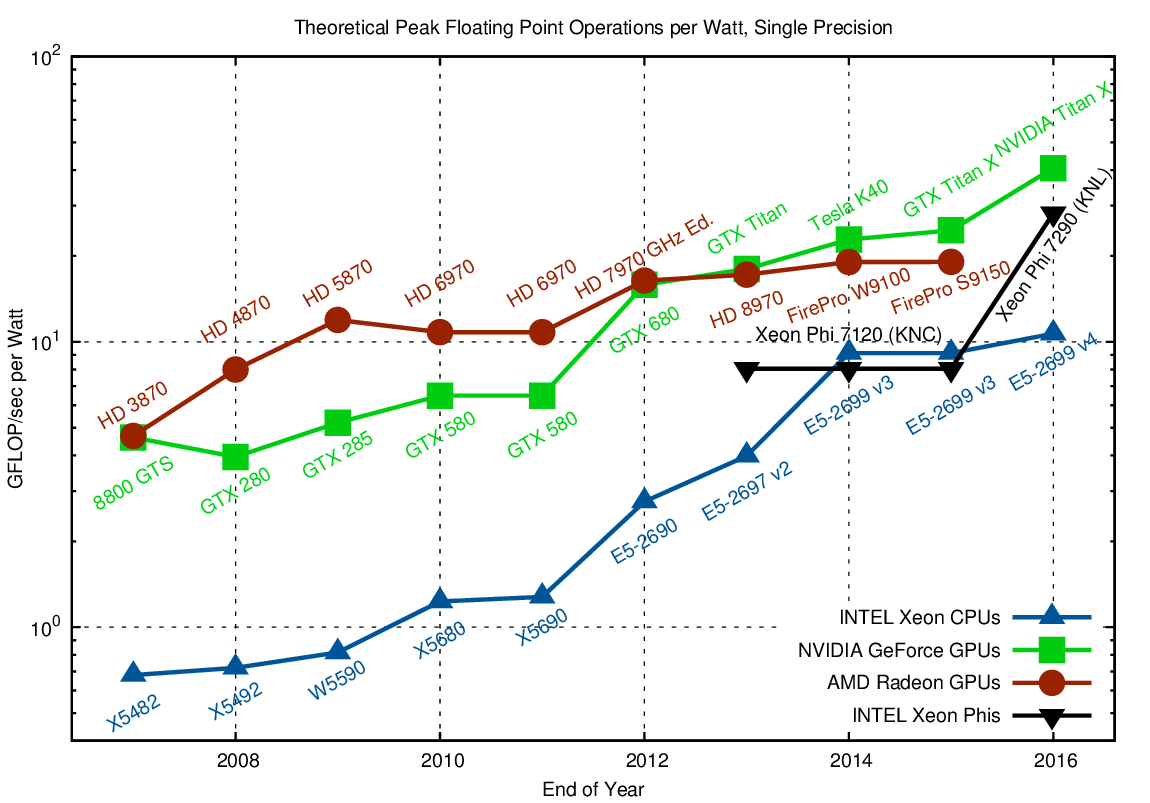
\includegraphics[width=1.0\textwidth]{./images/parallel_programming/gflops-per-watt-sp}
    	\caption[GFLOPs per \si{Watt} metric for CPUs and GPUs]{GFLOPs per \si{Watt}, Higher is better. GPUs offer higher performance per Watt utilised especially for those fine-grained massively parallel problems such as dense matrix-matrix multiplication. Note that the Figure also shows that the CPU is getting smaller, indicating that CPU are introducing more GPU-like capabilities into their transistors. \textit{Intel} added wider vector processing units (up to 64 byte) to their latest processors. }
    	\label{gflops-per-watt-sp}
    \end{figure}
  
    \subsection{From Graphics Graphics to General Purpose HW}\label{graphicPipeline}
    A graphics task such as rendering a $3D$ scene on the screen
    involves a sequence of processing stages inside the GPU, i.e. shaders, that run in parallel and in a prefixed order, known as the graphics hardware
    pipeline \cite{Shirley:2005:FCG:1088893} which is the most common form of 3D computer rendering, distinct from, for instance, \textit{raytracing} or \textit{raycasting} for which the concept of pipeline is not even defined.
     \begin{figure}[H]
    	\centering
    	\caption{Typical computer graphics pipeline.}\label{graphicPipeline}
    	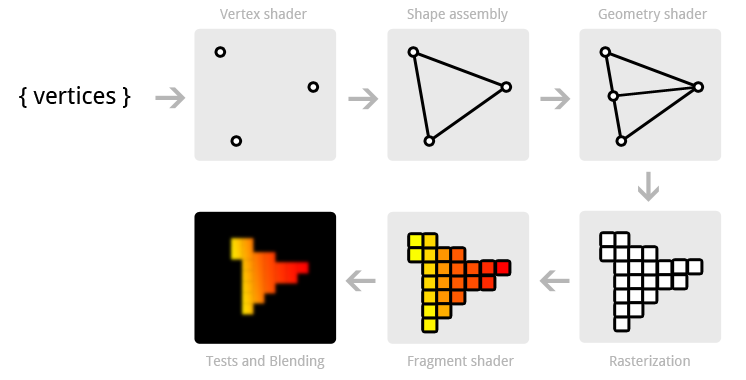
\includegraphics[width=1.0\textwidth]{./images/parallel_programming/pipeline}
    \end{figure}
    
     Figure \ref{graphicPipeline} shows the important key steps that make up the graphic pipeline and for which the GPU hardware has been specialized for years. The pipeline works taking as input graphics primitives, each stage forward its results on to the next stage.
    \begin{itemize}
    	\item     The first stage of the pipeline is the \textit{vertex shader}. The
    	input to this phase is a list of vertices in object space coordinate which are then converted to world coordinates (applying the \textit{model and view matrices}).
    	\item  Shape assembly is performed where vertices are grouped together by forming graphics primitives, i.e. lines, point, polygons, triangles, tringles strips etc. If enabled, lighting calculation are also performed for each vertex.
    	\item   The following step, the \textit{geometry shader} is optional in the \texttt{openGL} pipeline and can be used to produce or delete primitives. One of the most common use of this shader is in reducing the communication between the GPU and the CPU. For instance one can only pass to the graphic pipeline a list of vertices for drawing cubes, and produce the primitives for them only when the the geometry shader is executed, reducing the amount of information exchanged between the CPU and the GPU.
    	\item   Each of the (from the now final list of) primitives is scan-converted or rasterized generating a set of fragments in screen space for the visible only part of the shapes. Each fragment stores the state information needed to update a pixel and are obtained by interpolating per vertex attributes coming from the geometry shader. For instance, each vertex of a triangle end up having its color changed based on the the color of its neighbors. 
    	\item  In the \textit{fragment  shader} is used to calculate the final color of each individual fragment. Texture coordinates of each fragment are used to fetch colors of the appropriate texels (texture pixels) from
    	one or more textures. Further interpolation may also be
    	performed to determine the ultimate color for the fragment.
    	\item Finally, various tests (e.g., \textit{depth} and \textit{alpha}, etc.) are conducted to determine whether or how the fragment should be used to update a pixel in the frame buffer.    
    	Each shader in the pipeline performs a basic but specialised operation on the
    	vertices as it passes. 
    \end{itemize}

    In a shader based architecture the individual shader processors exhibit very limited capabilities beyond their specific purpose.
    Before the advent of CUDA in 2006 most of the techniques for non-graphics
    computation on the GPU took advantages of the programmable fragment processing stage. The steps involved in mapping a computation on the GPU are
    as follows:
    \begin{enumerate}
    	\item The data are laid out as texel colors in textures;
    	\item  Each computation step is implemented with a
    	user-defined fragment program. The results are encoded as pixel colors and rendered into a  pixel-buffer (stored into GPU main memory, similar to a frame-buffer); 
    	\item Results that are
    	to be used in subsequent calculations are copied to textures for temporary storage and the process could start over again for another iteration.
    \end{enumerate} 
    
    The year 2006 marked a significant turning point in GPU architecture. The \texttt{G80}  was the first \textsc{NVIDIA} GPU to have a unified architecture whereby the different shader processors were  combined into unified stream processors (see Figures \ref{fig:volta_sm} and \ref{fig:volta_architecture} at pages \pageref{fig:volta_sm}  \pageref{fig:volta_architecture} respectively). The resulting stream processors had to be more complex so as to provide all of the functionality of the shader processors they replace. Although research had been carried out into general purpose programming
    for GPUs previously, this architectural change opened the door to a far wider range of  applications and practitioners.
    GPUs are nowadays, well suited for data-parallel problems because they are very effective at executing the same code on many data elements at the same time  in a \textit{Single Instruction, Multiple Threads} (SIMT) fashion or using a more general definition as \textit{Parallel Random-Access Machine in which each thread Can Read or Write a memory location} (\texttt{CRCW PRAM}).
    
    
\section{The OpenCL Parallel Computing Paradigm on Heterogeneous Devices}
    Released on December 2008 by the Kronos Group, \texttt{OpenCL} \cite{Gaster:2011:HCO:2046379,Stone:2010:OPP:622179.1803953,Munshi:2011:OPG:2049883} is an open standard for programming heterogeneous computers built from CPUs, GPUs and other processors. It allows to define the intended computation using the \textit{platform} abstraction. A platform is composed by an host and one or more compute devices. A C-like language is used to program and orchestrate the various components of the platform (see Figure \ref{fig:openCL_platform}).
    
    One of the advantages of \texttt{OpenCL} is that it is not restricted, as in the case of CUDA\cite{NvidiaprogGuide}, to the use of GPUs only but it takes each computing resource in the system as computational peer unit, interposing a uniform set of API between them and the programmer, easing the process of interfacing with them. Another big advantage is that it is  open, free, and cross-compatible across vendors since is supported by all major hardware producers.
    
    A typical \texttt{OpenCL} application is subdivided in two parts, one
    running on the CPU (\textit{host} application) and one or more running on a
    compliant device (\textit{device} application), where the actual parallel
    computation generally takes place. The host application defines
    the tasks to be executed in parallel. Each parallel task is
    implemented as an \texttt{OpenCL} \emph{kernel}, which is a special C
    function, which is compiled at runtime for each specifically for and deployed to a compliant device, or to different ones, for execution. The execution model is similar to the one of CUDA (CUDA and OpenCL share a similar programming model and underlying hardware architecture, even if a quite different terminology is adopted), where each kernel is executed by \textbf{threads}, the smallest execution entity, also called \textbf{work-items}, which are grouped into \textbf{work-groups}. A work-item is executed by one or more processing elements as part of a work-group executing on a compute unit. A work-item has to be considered a thread in terms of its control flow and memory model, but the hardward and the compiler can run multiple work-items on a single thread. As an example one can imagine that work-items computation can be carried out on lanes of a SSE vector. 
    A work-group is a collection of related work-items that execute on a single compute unit. A work group must map to a single compute unit (a core on a CPU, or using CUDA terminology a streaming multiprocessor). 
    Work-groups can sunchronize internally between work-items using local or global memory or barriers but they cannot synchronize with each other, making impossible building locking and synchronization primitives (among work-groups).
    The  locality of execution of work-items  leads to more efficient synchronization, and makes possible to have access to user managed local fast memories and caches (similar to CPU L1 caches) in order to makes communication fast.    
    A work-item is distinguished from other executions within the collection by its \textbf{global ID} and \textbf{local ID} (relative to the parent worl-group).
    
    Work-groups can:
    \begin{itemize}
		\item \textbf{Share data} between the work-group's work-items using local memory
		\item \textbf{Synchronize} between work-items using barriers and memory fences mechanism
		\item \textbf{Use special built-in functions} such as \texttt{work\_group\_copy}
    \end{itemize}

    \begin{figure}
	\centering
	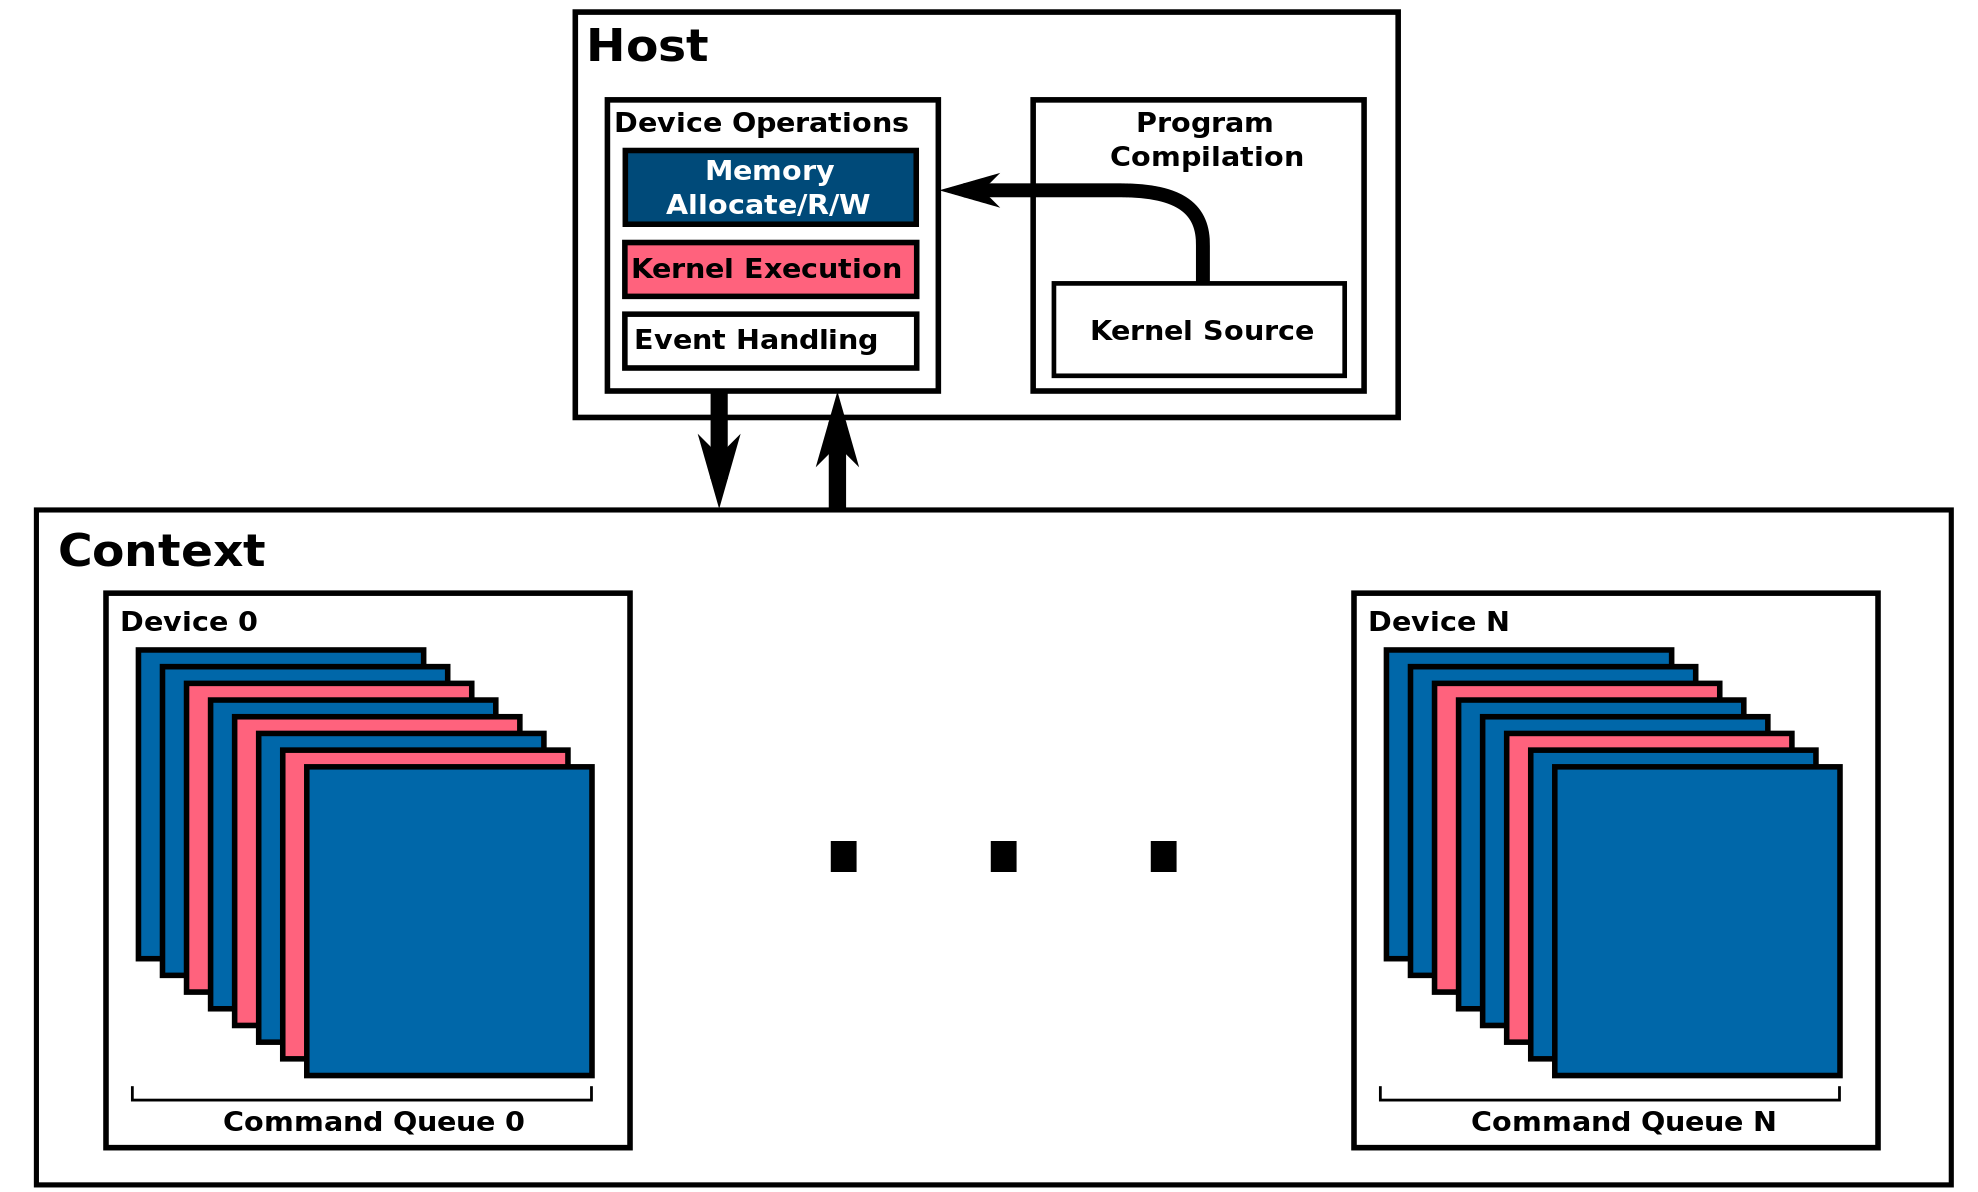
\includegraphics[width=1.0\textwidth]{./images/parallel_programming/openCL}
	\caption[\texttt{OpenCL} platform abstraction.]{\texttt{OpenCL} platform abstraction. A device is any supported device including GPU, CPU, FPGAs, etc.. Command queues are executed concurrently for each device and can be synchronized by means of API calls.}
	\label{fig:openCL_platform}
\end{figure}

    \begin{figure}
	\centering
	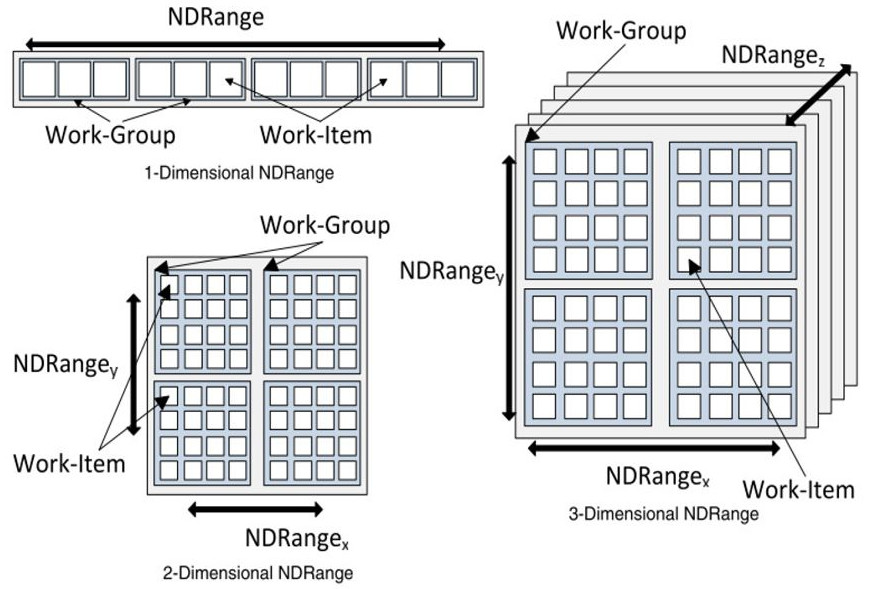
\includegraphics[width=0.85\textwidth]{./images/parallel_programming/opencl_execmodel}
	\caption{\texttt{OpenCL} 1D,2D,3D work-items and work-groups partitioning. }\label{fig:opencl_execmodel}
\end{figure}

	Work-groups and work-items are arranged in a indexed grid-like structure. 
    When launching the kernel for execution, the host code defines the grid dimensions, or the global work size. The host code can also define the partitioning to work-groups, or leave it to the implementation. During the execution, the implementation runs a single work item for each point on the grid (a kernel per work-item). It also groups the execution on compute units according to the work-group size. The order of execution of work items within a work-group, as well as the order of work-groups, is implementation-specific (see Figure \ref{fig:work_group_execution}).
    Data to be processed has to be explicitly partitioned and assigned to compute units because each work-item runs the same kernel on different portions of data in a \textit{SIMD/SIMT} fashion. For example, in case of an array of $n$ elements and $n$ work-items, data can be partitioned by associating each work item to the array element with index corresponding to the work-item global ID. Figure \ref{fig:opencl_execmodel} depicts how items and groups can be arranged when partitioned in $1D$, $2D$ and $3D$.
    Figure \ref{fig:opencl_execmodel2d} shows a $2D$ decomposition with details on global ID computation from local group and thread indices.
    
\begin{figure}[!htbp]
    	\centering
    	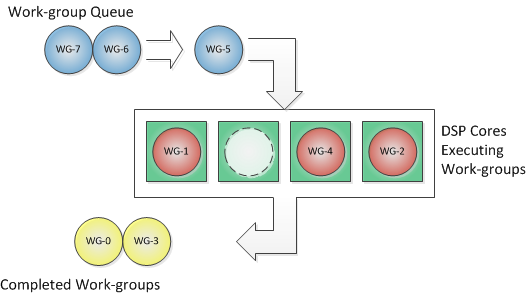
\includegraphics[width=0.85\textwidth]{./images/parallel_programming/work_group_execution.png}
    	\caption[\texttt{OpenCL} work group scheduling]{\texttt{OpenCL}  work-groups scheduling. 
    	The green boxes represent the computing unit. The circles represent the work-groups. Blue work-groups are waiting to be executed, pink work-groups are currently executing and yellow work-groups have been completed. Each work group is queued for execution and executes on a single computing unit (a GPU multiprocessor, CPU core, etc.) Note that execution order is not guaranteed by the standard.}
    	\label{fig:work_group_execution}
    \end{figure}

        \begin{figure}
    	\centering
    	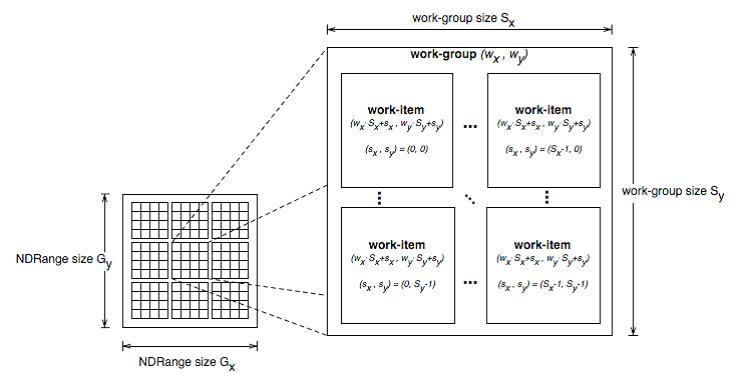
\includegraphics[width=1.1\textwidth]{./images/parallel_programming/opencl_execmodel2d}
    	\caption[\texttt{OpenCL} 2D work-items and work-groups detailed partitioning]{\texttt{OpenCL} 2D work-items and work-groups detailed partitioning. The computation of global index from local item and group index is also shown.}\label{fig:opencl_execmodel2d}
    \end{figure}
    When the kernel execution terminates,
    work-items globally synchronize, and the control returns to the
    host application. Similarly to the OpenMP fork-joins stages,
    different kernel executions and synchronization stages can take
    place in a typical \texttt{OpenCL} application.
    
    Data can be shared by all the running work-items by means of the
    device global memory, which is generally the largest among all the
    different memory levels available on the device (this is especially true for modern GPUs)
    though being the slowest. A read-only memory, equivalent to the
    global one in terms of latency and dimension, called constant
    memory, is also available. Some devices have an appropriate
    portion of this memory, while in other cases the constant memory
    space coincides with that of the global memory. Threads within a
    work-group are executed by a specific compute unit and therefore
    can share data on the local memory and also synchronize each
    other. Local memory is generally smaller with respect to the
    global one, but allows for faster access (about $100\times$ faster
    on modern GPUs). Eventually, each work-item has its own private
    memory, which is at the same time the fastest and the smallest
    one. 
    
    The memory in which a given data is stored must be
    initially defined and allocated by the host using the appropriate API calls (e.g. see Listing \ref{code:opencl_allocate}). 
    \lstset{language=[OpenCL]C,
    	basicstyle=\ttfamily,
    	caption={Allocate buffer API call in OpenCL.},
    	label={code:opencl_allocate},
    	morekeywords={cl_context,clCreateBuffer,cl_mem_flags,cl_int,size_t},
    	keywordstyle=\color{ultramarine}\ttfamily,
    	stringstyle=\color{rosemadder}\ttfamily,
    	commentstyle=\color{outerspace}\ttfamily,
    	backgroundcolor=\color{white}, 
    }
    \begin{lstlisting}
		clCreateBuffer(cl_context context,	cl_mem_flags flags,
						size_t size,void *host_ptr,cl_int *errcode_ret)
    \end{lstlisting}
  	 Nevertheless, data can move among different memory levels during kernel execution (from global, to local, to private or the other way round).
    
    Data exchange and kernels execution are managed by the host thanks
    to an \texttt{OpenCL} context. In particular, the host application links
    kernels into one or more containers, called \emph{programs}. The
    program therefore connects kernels with the data to be processed
    and dispatches them to a special \texttt{OpenCL} structure called
    \emph{command queue} (see Figure \ref{fig:openCL_platform}). This is necessary because only enqueued kernels are actually executed.
    The context contains all the
    devices, command queues and kernels, whereas each device has its own
    command queue each containing the kernels to be
    executed on the corresponding device. Moreover, an \texttt{OpenCL}
    application can configure different devices to perform different
    tasks, and each task can operate on different data. \texttt{OpenCL}
    is thus capable of full task-parallelism. Command queues are also
    used for host-device and device-device data transfer operations,
    synchronization between different kernels, and profiling
    operations.
    
    
	Kernels are usually listed in separate
    files the \texttt{OpenCL} runtime use to create kernel object that
    can be first decorated with the parameters on which it is going to
    be executed and then effectively enqueued for execution onto device.
    
    The following is a brief description of the typical flow of an \texttt{OpenCL} application (See Figure \ref{fig:opencl_execmodel}).
    \begin{figure}
    	\centering
    	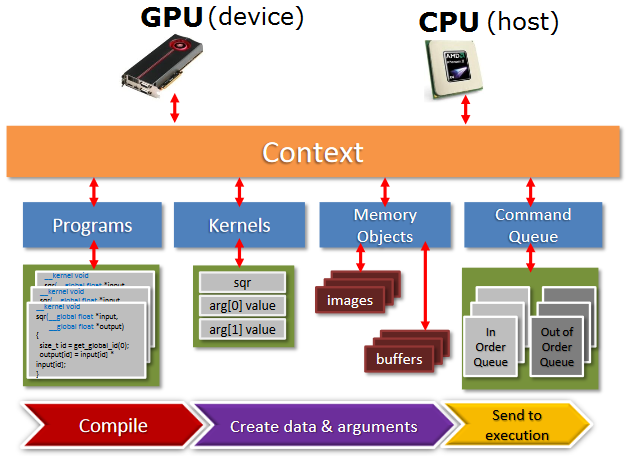
\includegraphics[width=1.0\textwidth]{./images/parallel_programming/opencl_program_flow}
    	\caption{\texttt{OpenCL} program flow and interaction between memory, device and host.}\label{fig:opencl_execmodel}
    \end{figure}

    \begin{description}
    	\item [Contexts creation:]\hfil \\ The first step in every \texttt{OpenCL} application is to create a context and associate to it a number of devices, an available \texttt{OpenCL} platform (there might be present more than one implementation). Each subsequent operation (memory management, kernel compiling and running), is performed within \emph{this} context. In the example \ref{code:openCLContext} a context associated with the CPU device and the first platform returned by OpenCL is created.
    	\lstset{language=[OpenCL]C,
    		caption={\texttt{OpenCL} Context Creation.}, 
    		label={code:openCLContext}, 
    		basicstyle=\ttfamily,
    		keywordstyle=\color{ultramarine}\ttfamily,
    		morekeywords={cl_context,clCreateBuffer,cl_mem_flags,cl_int,size_t},
    		stringstyle=\color{rosemadder}\ttfamily,
    		commentstyle=\color{outerspace}\ttfamily,
    		backgroundcolor=\color{gray!5}, 
    		numbers=left, 
    		numberstyle=\tiny
    	}
    	\begin{lstlisting}
    	cl_int err;
    	cl::vector<cl::Platform> platformList;
    	//Gets a list of available platforms.
    	cl::Platform::get(&platformList); 
   		checkErr(platformList.size()!=0 ?CL_SUCCESS:-1,"cl::Platform::get");
    	cl_context_properties cprops[3] ={CL_CONTEXT_PLATFORM,(cl_context_properties)(platformList[0])(), 0};
    	//create a context based on the first platform from the list
    	//Constructs a context including a list of specified devices
    	cl::Context context(CL_DEVICE_TYPE_CPU,cprops,NULL,NULL,&err);
    	check_error(err, "Conext::Context()"); 
    	\end{lstlisting}

    	\item [Memory buffers creation:]\hfil \\ \texttt{OpenCL} buffer objects on which kernels operates are created at this point using an available and valid context object as shown in Listing \ref{code:opencl_buffer_creation}. 
    	\lstset{language=[OpenCL]C,
    		caption={\texttt{OpenCL} context creation}, 
    		label={code:opencl_buffer_creation}, 
    		keywordstyle=\color{ultramarine}\ttfamily,
    		morekeywords={cl_context,clCreateBuffer,cl_mem_flags,cl_int,size_t},
    		stringstyle=\color{rosemadder}\ttfamily,
    		commentstyle=\color{huntergreen}\ttfamily, 
    		backgroundcolor=\color{gray!5}, 
    		numbers=left, 
    		numberstyle=\tiny
    	}
    	\begin{lstlisting}
    	memobj = clCreateBuffer(context, CL_MEM_READ_WRITE,MEM_SIZE * sizeof(char), NULL, &ret);
    	check_error(err, "Buffer::Buffer()");
    	\end{lstlisting}
    	
    	\item [Build a program:]\hfil \\ 
    	The actual code that runs on the devices has to be compiled first. The \textbf{\textit{cl::Program}} object takes care of building the device code for the devices listed during the context creation. See Listing
    	\ref{code:loadBuildProgramCL} for an example of how \textbf{\textit{cl::Program}} are created.
    	     \lstset{language=[OpenCL]C,
    		caption={\texttt{OpenCL} program load and build}, 
    		label={code:loadBuildProgramCL}, 
    		keywordstyle=\color{ultramarine}\ttfamily,
    		morekeywords={cl_context,clCreateBuffer,cl_mem_flags,cl_int,size_t},
    		stringstyle=\color{rosemadder}\ttfamily,
    		commentstyle=\color{outerspace}\ttfamily,
    		backgroundcolor=\color{gray!5}, 
    		numbers=left, 
    		numberstyle=\tiny
    	}
    	\begin{lstlisting}
    	std::ifstream file("pathToSourceCode.cl");
    	check_error(file.is_open() ? CL_SUCCESS:-1, "pathToSourceCode.cl");std::string
    	prog( std::istreambuf_iterator<char>(file),
    	(std::istreambuf_iterator<char>()));
    	cl::Program::Sources source(1,std::make_pair(prog.c_str(), prog.length()+1));
    	cl::Program program(context, source);
    	err = program.build(devices,"");
    	check_error(err, "Program::build()");
    	cl_kernel kernel = clCreateKernel(program, "nameofthekernel", &ret);
    	\end{lstlisting}
    	
    	
    	\item [Kernel launch:]\hfil \\
    	In order a kernel to be executed a \emph{kernel object} must be created.
    	For a given \emph{Program} there would exists more than one entry point
    	(identified by the keyword \emph{\_\_kernel}. We choose one of them for
    	execution specifying its name in the kernel object constructor.    	
    	 We effectively execute the kernel putting it into a 
    	\emph{cl::CommandQueue}. Given a cl::CommandQueue queue, kernels can be queued
    	using \textit{queue.enqueu\-NDRangeKernel} that queues a kernel on
    	the associated device.
    	Launching a kernel need some parameters (similar to launch configuration in
    	\texttt{CUDA}) to specify the work distribution among
    	work-groups and their dimensionality and size of each dimension (see listing
    	\ref{code:openCLQueuCommand}). We can test the status of the execution by
    	querying the associated \emph{event}.
    	    \lstset{language=[OpenCL]C,
    		caption={\texttt{OpenCL} command queue definition and kernel enqueuing.}, 
    		label={code:openCLQueuCommand}, 
    		keywordstyle=\color{ultramarine}\ttfamily,
    		morekeywords={cl_context,clCreateBuffer,cl_mem_flags,cl_int,size_t},
    		stringstyle=\color{rosemadder}\ttfamily,
    		commentstyle=\color{outerspace}\ttfamily,
    		backgroundcolor=\color{gray!5}, 
    		numbers=left, 
    		numberstyle=\tiny
    	}   
    	\begin{lstlisting}
    	cl::CommandQueue queue(context, devices[0], 0, &err);
	    /*cl_kernel kernel = clCreateKernel(program, "nameofthekernel", &ret);*/
	    kernel.setArg(0,memobj);
	    //let the work-group size be choosen by the implementation 
	    ret = clEnqueueNDRangeKernel(queue, kernel, 1, NULL,
	    &MEM_SIZE, NULL, 0, NULL, NULL)
    	\end{lstlisting}
    \end{description}
\end{description}
 
%%%%%%%%%%%%%%%%%%%%%%%%%%%%%%%%%%%%%%%%%%%%%%%%%%%%%%% 
%\subsection{The Message Passing Interface}
